\documentclass{article}[12pt, openright, oneside, a4paper, portuguese]
\usepackage[utf8]{inputenc}
\usepackage[brazil]{babel}
\usepackage{graphicx}
\usepackage{hyperref}
\usepackage[top=3cm,bottom=2cm,left=3cm,right=2cm]{geometry}
\usepackage{indentfirst}
\usepackage{cite}
\usepackage{src/ABNT/abnt-alf}
\usepackage{float}
\usepackage{tikz}

\begin{document}
% CAPA
\pagestyle{empty}
\begin{figure}
    \centering
    \includegraphics[width=0.35\linewidth]{src/Imagens/escola_politecnica_0.jpg}
\end{figure}
\begin{center}
\large{
\textbf{REDES NEURAIS ARTIFICIAIS APLICADAS A GARANTIA DE ESCOAMENTO MULTIFÁSICO DE PETRÓLEO E GÁS}

\vspace{0.5cm}
HISTORICIZAÇÃO E CONTEXTUALIZAÇÃO
}

\vspace{2cm}
\large{\textbf{Guilherme Silva Freire\textsuperscript{1}}}

\vspace{1cm}
\textsuperscript{1} Escola Politécnica\\
Universidade Federal da Bahia\\
Salvador–BA-Brasil\\

\vspace{1cm}
\href{mailto:guilhermefreire@ufba.br}{guilhermefreire@ufba.br}

\vspace{2cm}
\large{
ENGG23: Tópicos Especiais em Engenharia de Controle e Automação\\
Introdução ao Petróleo\\
\vspace{1cm}
Prof.: Leonardo Silva de Souza
}\\

\vspace{2cm}
\large{\textbf{SALVADOR 2024}}
\end{center}

% RESUMO
\newpage
\Large{\textbf{Resumo}}

	A utilização de Redes Neurais Artificiais (RNAs ou ANNs) para a otimização de processos na indústria cresce constantemente, por conta da sua capacidade de modelar funções não-lineares complexas. A otimização utilizando redes neurais tem como ideia central substituir os modelos já utilizados, que apresentam diversos problemas relacionados a convergência e restrições, e ter a possibilidade de mapear toda a função objetivo para que assim, possam se calcular diversos pontos ótimos \cite{NASCIMENTO20002303}. Na indústria do Petróleo, o escoamento é um dos principais fatores que determina os custos e a produção, entretanto esse campo apresenta diversos desafios, como o surgimento de hidratos, golfadas, asfaltenos entre outros. Como dito anteriormente, as RNAs serão aplicadas para otimizar e facilitar as previsões do \textit{flow assurance}, podendo, também, ser escalada para outras áreas da indústria, como extração e distribuição. Os dados utilizados para alimentar a rede virão de um simulador pré-existente, no caso dessa pesquisa, o ALFASIM. Como resultado, se espera alcançar uma rede neural que consiga prever futuras quadros e situações em certa rede de escoamento de petróleo e gás.

    \textbf{Palavras-chave:} RNAs, Indústria de Petróleo, Flow Assurance, Previsão, Otimização de Processos

% Introdução
\section{Introdução}

    A indústria do Petróleo se encontra presente no dia a dia de toda população mundial. O Petróleo, é uma matéria-prima que pode determinar o futuro de países e da economia mundial, diversas sociedades dependem do mercado como fonte de renda principal, como, por exemplo, os Emirados Árabes. A indústria de petróleo pode ser dividida em exploração, escavação, produção e transporte \cite{Solomon2024}, nesse artigo falaremos principalmente sobre a produção e a otimização do escoamento multifásico.
    
    No Brasil, a produção de petróleo apresenta diversas dificuldades, pois as reservas apresentam óleo pesado, o qual é mais denso e viscoso, essas características representam uma grande limitação de produção, já que o entupimento dos canos, corrosão e erosão são mais propensos a acontecer, ademais, a força das bombas e a separação de fases somatizam ainda mais a dificuldade de coleta e refino. A solução desses problemas representa um gasto excessivo em mão de obra e materiais extras, esse gasto aumenta em várias vezes se é pensado para pontos de coleta \textit{Offshore}, especificamente no pré-sal. Pensando nisso, a otimização do escoamento se torna obrigatória, visto que a prevenção aos danos viabiliza uma solução sem cortes na produção.
    
    As redes neurais são algoritmos capazes de aprender a solucionar as funções objetivos apresentadas, sendo amigáveis com restrições e sistemas complexos, como, por exemplo, as equações de \textit{Navier-Stokes} para mecânicas dos fluidos. A principal vantagem da utilização de RNAs é a previsão de situações futuras sem precisar alterar a rede neural em si, apenas um treinamento eficiente já é escalável para diversos problemas similares, com restrições e pontos iniciais diferentes. Essa vantagem se dá principalmente porque a rede não precisa modelar as equações físicas e químicas que envolvem o sistema, entretanto a aplicabilidade desses modelos não deixa de existir, pois os seus usos podem diminuir a quantidade de dados necessários para a RNA ter um bom desempenho.


% Sobre o Autor
\section{Sobre o autor}

    Guilherme Silva Freire nasceu em Feira de Santana, chegou à UFBA em busca de conhecimento e vivências. Durante a adolescência, semp're foi incentivado a participar de olimpíadas e competições de conhecimento, conquistando medalhas ao nível nacional. Essas experiências não apenas lhe trouxeram reconhecimento, mas também fortaleceram seu comprometimento e dedicação. 
    No Ensino Médio, começou a dar aulas de matemática e física como professor autônomo, enquanto se preparava para o vestibular. Conseguiu ser aprovado no curso de Engenharia de Controle e Automação na UFBA em 2023.1, entretanto inicialmente ele tinha planos para cursar Engenharia Mecatrônica na UNICAMP ou USP, mas optou por ficar na Bahia, por conta do interesse na área de Petróleo Offshore. Na universidade, adentrou na Empresa Júnior do curso, onde esperava obter conhecimento e experiência na área de Automação, nesse mesmo período, fez diversos cursos sobre controle de sistemas e ainda tem diversos outros cursos para começar.
    Após terminar a graduação pleiteia seguir carreira acadêmica ou prestar concurso para a Petrobrás. No fim da carreira deseja focar totalmente em desenvolvimento de pesquisas, seja na UFBA ou em outras faculdades.

% Desenvolvimento 1
\section{Escoamento multifásico na Indústria de Petróleo}

    \textit{Flow assurance} é o campo de pesquisa que visa a garantia de produção de óleo e gás através da mitigação das restrições do fluxo do fluido, esse campo de desenvolvimento tem raízes no programa tecnológico PROCAP 1000 \cite{Freitas1999}, da Petrobrás, que obteve como fruto mais de 250 patentes significantes.
    
    Na indústria o escoamento multifásico é vítima de diversos problemas, sendo eles principalmente bloqueios e restrições em toda rede de poços e canos. De acordo com \citeonline{makogon2019handbook} as restrições podem ser hidráulicas, como acumulação de líquido em curvas, podendo causar engasgos e golfadas, mecânicas, como uma válvula meio-aberta, e sólidas, como o surgimento de sólidos orgânicos, inorgânicos ou partículas. Os tipos de restrições mais difíceis de prever são as hidráulicas e sólidas, já que dependem do quadro PVT (Pressão-Vazão-Temperatura) do fluido e da tubulação em si, a análise dessas características, a partir de uma boa modelagem, permite o engenheiro fazer previsões e alterações no \textit{design} do poço, identificando quais tecnologias serão necessárias, sempre visando o menor custo.

    Os principais desafios e obstáculos do escoamento são revisados em \citeonline{Muhammad2018}, sendo eles, seus tipos e suas causas listadas a seguir:
    
    \begin{center}
    \begin{tabular}{||p{4cm}|p{3cm}|p{8cm}||}
    \hline
    Problema & Tipo & Causa \\
    \hline
    Hidratos & Sólido & Alta pressão e baixa temperatura \\
    Deposição de Parafina & Sólido & Baixa temperatura na parede da tubulação \\
    Asfaltenos & Sólido & Má manipulação do PVT e mudança da composição das fases \\
    Golfadas ou Gargalos & Hidráulico & Bloqueio da passagem de gás pelo líquido em curvas verticais \\
    Naftenatos & Sólido & Precipitação de ácidos Naftênicos, resultantes do processamento de produtos do petróleo \\
    \hline
    \end{tabular}
    \begin{tabular}{||p{4cm}|p{3cm}|p{8cm}||}
    \hline
    Problema & Tipo & Causa \\
    \hline
    Escamas & Sólido & Formação de depósitos de sais e óxidos insolúveis pelo escoamento da água \\
    Erosão & Mecânico & Partículas sólidas arranham as paredes de equipamentos e tubos \\
    Emulsões & Sólido & Devido a baixas temperaturas e a viscosidade dos fluidos, podem ocorrer diversos tipos de emulsões, dificultando a separação de fases\\
    \hline
    \end{tabular}
    \end{center}

    As principais formas de remediação de sólidos são: a inserção de inibidores ou dispersantes químicos e controle de temperatura, entretanto essa inserção passa a ter um custo alto devido à quantidade e estratégias de inserção dos químicos e quando é pensado na criação e aplicação de um controlador de temperatura ou o uso do método de Cold Flow \cite{Garcia2008}. Também é utilizada como manutenção a ferramenta PIG para desobstrução e detecção de problemas nos canos, porém, muitas vezes, a produção naquele tubo precisa ser parada.

    Para o principal problema hidráulico, a golfada, a principal estratégia é a utilização de \textit{gas-lift}, captadores de golfadas e sistemas inteligentes de mitigação e controle. Porém, esses métodos necessitam de grande investimento em pesquisa e instalação, aumentando os custos e exigindo a parada de produção. Para erosões, uma das soluções é a diminuição de curvas no \textit{pipeline}, já que ocorrem, na maioria das vezes, em curvas e quinas, esse método de resolução exige maior atenção antes de projetar o poço e deve ser evitado a qualquer custo, pois, o seu agravamento leva à substituição das áreas afetadas.

    A melhor forma de evitar a maioria os problemas citados é com um controle preditivo eficiente e inteligente, buscando sempre otimizar o sistema considerando toda a tubulação do poço e suas propriedades físicas. Logo, a modelagem eficiente de um poço, com a ferramenta ALFASIM, por exemplo, utilizando a otimização do sistema por redes neurais, se torna um meio barato e eficiente para solucionar a lacuna de controle preditivo.

% Desenvolvimento 2
\section{Redes Neurais Artificiais na Indústria de Petróleo}

    A otimização em processos industriais se caracteriza pela busca do quadro mais eficiente para dado objetivo, evitando perdas e se mantendo nas condições restritivas. Existem diversas estratégias de otimização, \citeonline{Carson1997} trazem uma análise crítica entre os principais métodos e demonstram as suas aplicações em simulações. Os métodos possibilitam refinar os sistemas de simulação a cada iteração, trazendo um \textit{feedback} sobre a proximidade com os resultados esperados e fazendo as alterações necessárias na simulação, nas RNAs os otimizadores mais utilizados são os “Métodos de Procura Baseado no Gradiente”, como, por exemplo, o ADAM, as alterações que os métodos induzem ocorrem nos pesos e bias da rede.

    A escolha correta de uma rede neural deve sempre considerar a natureza do sistema em questão, já que ela é essencial para determinar a natureza da solução, a seguir são pontuados alguns exemplos de diferentes redes aplicadas a diversas áreas da indústria, com ênfase na indústria petrolífera.

    \subsection{RNA Comum}

     A figura 1 contém um diagrama de uma RNA simples, com duas entradas \boldmath{$x_1$} e \boldmath{$x_2$} e uma saída \boldmath{$y$}, a rede também contém duas camadas escondidas (\textit{hidden layers}). Os parâmetros que serão otimizados são os pesos \boldmath{$w$} e os bias \boldmath{$b$}. Cada camada na rede tem a sua função de ativação \boldmath{$\sigma$}. 

    \begin{figure}[H]
        \centering
        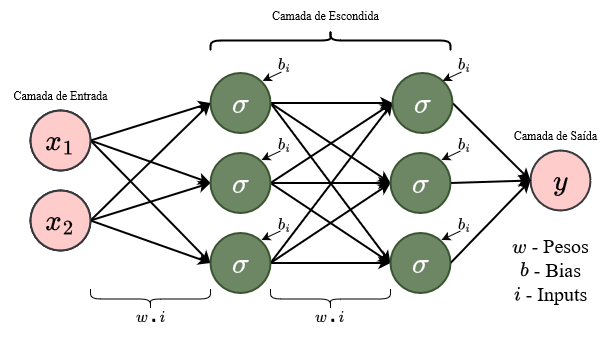
\includegraphics[width=0.5\linewidth]{src/Imagens/RNA Diagrama.drawio.png}
        \caption{Rede Neural Artificial Simples}
        \label{fig:enter-label}
    \end{figure}

    \begin{center}
        $ \sigma(wi + b)$ (1)
    \end{center}

    Os outputs de cada camada seguem (1) para entrar na próxima camada, por fim, a função de perda irá avaliar quanto cada peso e bias altera no resultado (através da técnica de \textit{back-propagation} e o compara com o resultado esperado, e assim, eles serão alterados de acordo com o resultado da comparação e sua influência.

    \citeonline{ELABBASY201450} desenvolveu uma rede neural para predizer as condições do \textit{pipeline}, buscando evitar corrosões, problemas mecânicos, erros operacionais entre outros. A identificação desses fenômenos é de alta dificuldade em águas profundas, devido à falta de instrumentos de coleta de informação. A rede neural promove uma melhor avaliação do estado da tubulação de um determinado poço, assim, permitindo os engenheiros tomar as medidas necessárias para evitar falhas críticas em pontos de coleta \textit{Offshore}.

    \subsection{PINN}
    
    As \textit{Physics Informed Neural Networks} (PINNs) são redes neurais que consideram o sistema do fenômeno físico para a sua aplicação, utilizando algoritmos de derivação automática para modelar o sistema e aplicá-lo na função de perda da rede. A maior vantagem da utilização de PINNs é o fato que não são necessárias grandes amostras de dados experimentais, necessitando essencialmente apenas das condições iniciais do sistema \cite{Blechschmidt2021}. A figura 2 representa uma PINN, deixando em evidência a sua camada de derivação automática e como a função \textit{Loss} interage com o sistema.
    
    \begin{figure}[H]
       \centering
        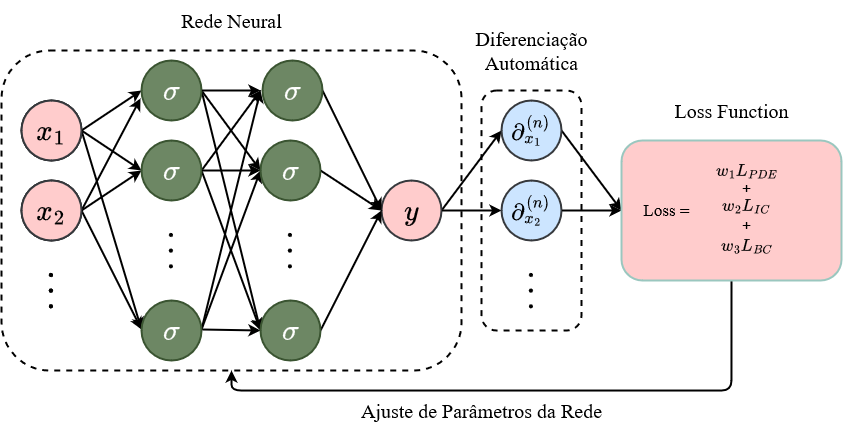
\includegraphics[width=0.75\linewidth]{src/Imagens/PINN DIAGRAMA.drawio.png}
        \caption{\textit{Physics Informed Neural Networks}}
    \end{figure}

    A análise de \citeonline{Cai2021} mostra que a utilização de PINNs pode se mostrar mais eficaz que os métodos numéricos convencionais para mecânicas dos fluidos, na análise se demonstra a aplicação em fluidos compressíveis, incompressíveis e biomédicos. Em cada exemplo é denotado a fidelidade com os dados experimentais coletados previamente, demonstrando melhor eficiência que outros algoritmos como solucionadores baseados em \textit{computional fluid dynamics} (CFD), por ter a capacidade solucionar sistemas de diversas dimensões com pouca quantidade de dados.

    \subsection{CNN}

    \textit{Convolutional Neural Network} (CNNs) são redes que aprendem e extraem dados a partir de \textit{forward} e \textit{backward propagation}, esse tipo de rede é normalmente aplicado na área de visão computacional e identificação de imagens. Na figura 3 é possível ver a construção de uma rede CNN, desde a sua separação de dados até sua função de propabilidade de escolha.

    \begin{figure}[H]
        \centering
        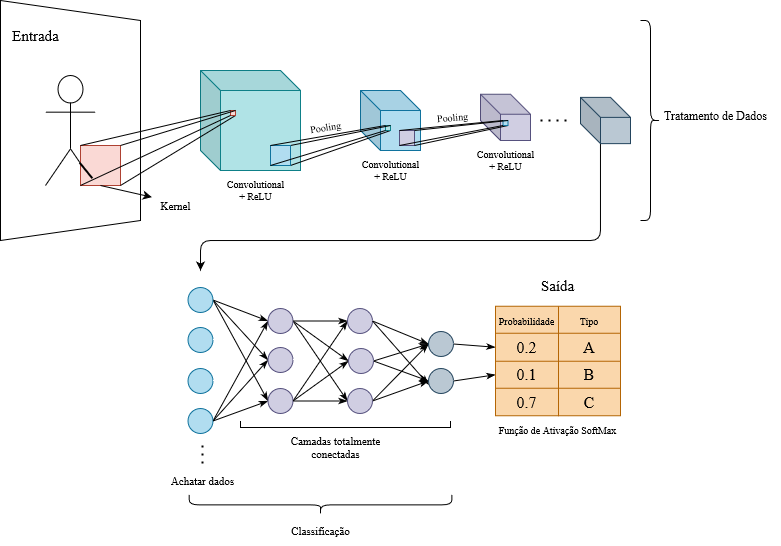
\includegraphics[width=0.75\linewidth]{src/Imagens/CNN Diagrama.drawio.png}
        \caption{\textit{Convolutional Neural Network}}
    \end{figure}
    
    \citeonline{QIAO2024104167} utiliza de uma rede de múltiplas CNNs para identificar padrões do escoamento multifásico em seções verticais do \textit{pipeline} a partir das vibrações do mesmo. Os dados são coletados por quatro sensores de vibração e tratados pela técnica de \textit{continuous wavelet transform} (CWT) e, assim, transformados em imagens, depois desse momento são enviados para quatro redes \textit{LeNet} e concatenados em apenas uma saída para fazer a previsão, a fusão de todos esses aspectos cria a CNN \textit{CWT-Mul-LeNet} usada na pesquisa. A precisão da identificação dessa rede chega a ser de 99,06\%.

    \subsection{RNN}

    Mais robustas do que redes neurais comuns, por conta da sua capacidade de memória para armazenar informação, as \textit{Recurrent Neural Networks} (RNNs), conseguem entender comportamentos não-lineares mais complexos. As RNNs são normalmente usadas para prever futuras situações do sistema, as redes são alimentadas com os dados variando no tempo (i.e. $X_{t-1}$ e $X_t$) para prever um dado futuro (i.e. $X_{t+1}$). Na figura 4, é representada este tipo de rede neural, sendo \boldmath{$x$} os dados de entrada, \boldmath{$h$} os dados de saída, \boldmath{$o$} a função de perda e \boldmath{$U, V, W$} os pesos.

    \begin{figure}[H]
        \centering
        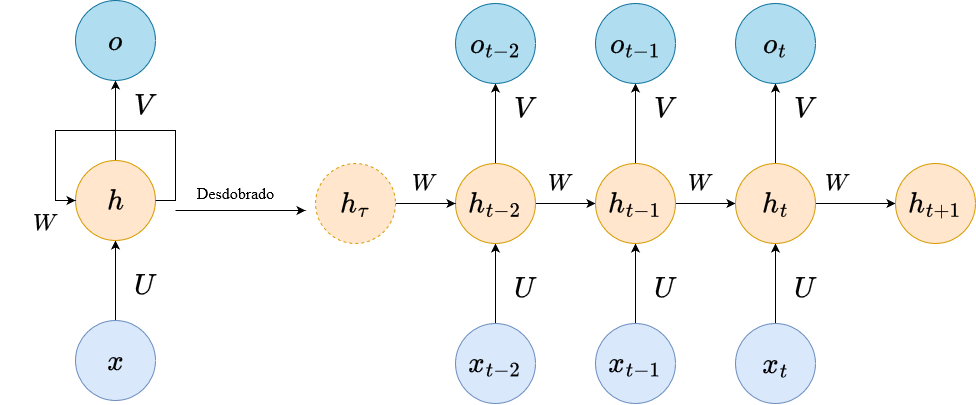
\includegraphics[width=0.75\linewidth]{src/Imagens/RNN DIAGRAMA.drawio.png}
        \caption{Recurrent Neural Network}
    \end{figure}

    Na pesquisa de \citeonline{ALKINANI2021100047} foi desenvolvido uma rede neural recorrente para fazer a regressão da função para prever a taxa de escavação em poços, os dados foram coletados em mais de 2000 poços escavados ao redor do mundo, que foram divididos entre dados de treinamento (entrada), validação (saída) e teste. A rede criada conseguiu prever um R\textsuperscript{2} médio de 0,94, conforme os pesquisadores, com esse método de predição, empresas do ramo de petróleo para efetuar melhor o controle dos parâmetros que afetam a taxa de escavação.

% Conclusões e resultados esperados
\section{Conclusões e resultados esperados}

    Esse trabalho tem como principal foco revisar a bibliografia sobre o uso e as vantagens da inteligência artificial na indústria do petróleo, dando ênfase no escoamento multifásico. É possível perceber que o uso de métodos mais atuais e específicos para cada situação se demonstra muito mais eficiente se comparado a métodos numéricos comuns. Como demonstrado em \citeonline{Cai2021}, diversos \textit{frameworks} já estabelecidos na indústria podem ser atualizados ou substituídos com a utilização de RNAs. Como objetivo final da pesquisa, os dados serão coletados a partir de programas de simulação de redes de petróleo, como o ALFASIM, a partir disso, é esperado criar uma rede neural para conseguir prever os possíveis problemas apresentados na seção 3, fiscalizando o estado do fluido multifásico e assim ser possível tomar as medidas necessárias para a prevenção ou remediação.

% Apêndices\
\def\refname{Referências Bibliográficas}
\bibliography{src/bibProj}
\bibliographystyle{src/ABNT/abnt-alf}
\addcontentsline{toc}{section}{Referências Bibliográficas}

\end{document}
